% Условная компиляция для самостоятельной работы
\ifdefined\mainfile
    % Если это часть основного файла, не добавляем начало и конец документа
\else
    \documentclass[12pt, a4paper]{report}
    \usepackage{/Users/vladbelousov/Desktop/Semestr_4-FP-NSU/Настройка/library}
    \usepackage[utf8]{inputenc} % Подключение поддержки UTF-8
    \begin{document}
\fi

%%-------------------------------%%
\section{Релятивистски инвариантное (ковариантное) описание электромагнитной волны}

\textit{Лоренц}  (1903-1904 гг) обнаружил линейное преобразование уравнений Максвелла, в движущиеся ИСО, не изменяющее вид этих уравнений. Это дало толчок в развитии теории относительности. \\

\textbf{Преобразование Лоренца:}  

\begin{center}
    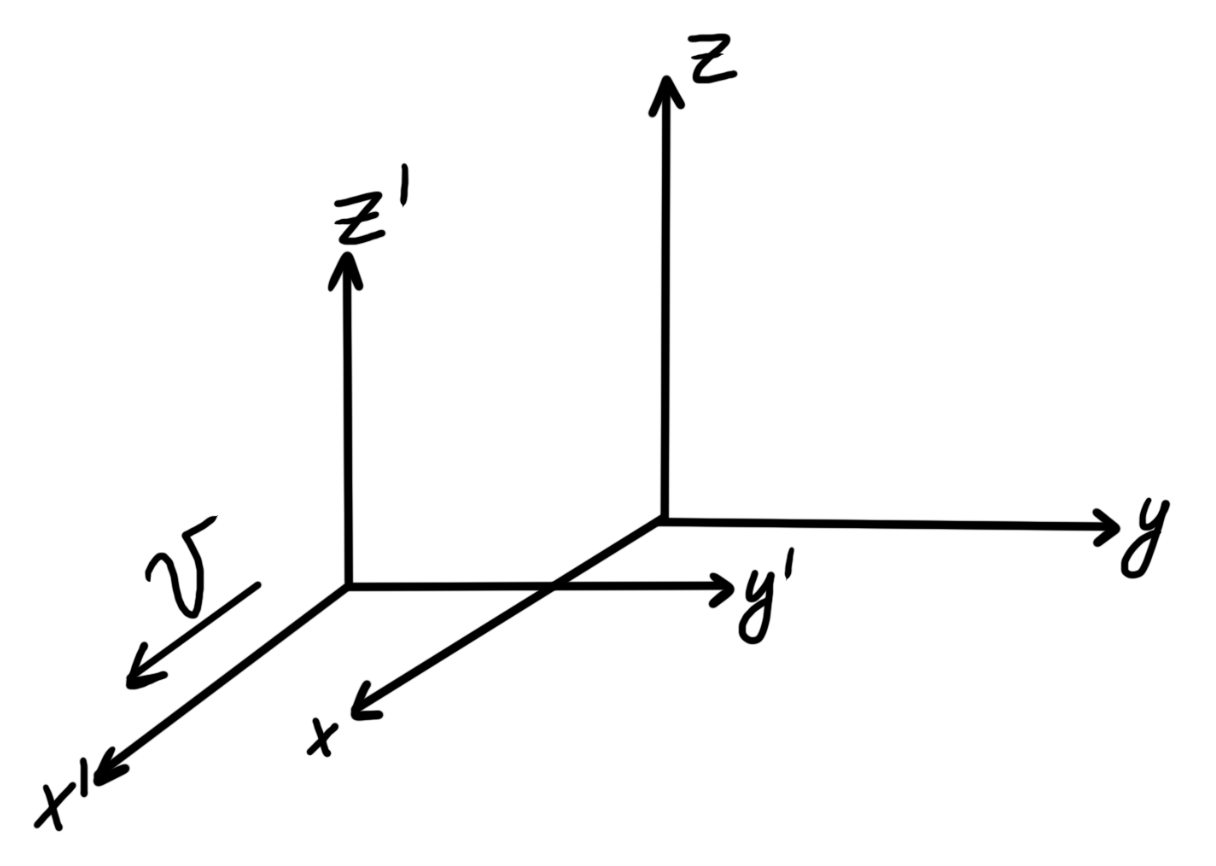
\includegraphics[width=0.6\textwidth]{/Users/vladbelousov/Desktop/Semestr_4-FP-NSU/ЭиО/Лекции_по_дням/image/178.png}
\end{center}

Координаты и время события при переходе из одной инерциальной системы отсчета (ИСО) в другую, движущуюся относительно первой постоянной скоростью \( v \), преобразуются следующим образом: 

\[ \begin{aligned}
\begin{cases}
c t ' = \gamma (ct - \beta x ) \\ 
x ' = \gamma (x - \beta ct ) \\ 
y ' = y \\ 
z ' = z \\ 
\end{cases}
\begin{cases}
ct = \gamma (c t ' + \beta x ' ) \\ 
x = \gamma (x ' + \beta ct ) \\ 
y = y ' \\
z = z' 
\end{cases}
\text{, где } \beta = \frac{v}{c }  , \text{ }  \gamma = \frac{1}{\sqrt{1 - \beta ^2 } }  
\end{aligned} \] 

\[ \vec{x }  = (ct , x , y ,z ) =(x^0 , x^1 , x^2 ,x^3 )= x^i  \] 

Правило: латинскими буквами \( (i , j  , k , l ,m ... ) \)  обозначают  индексы четырех мерных объектов = \( (0, 1, 2 ,3) \), а греческими \( (\alpha , \beta , \gamma , \delta ,... = 1,2,3) \) индексируют трех мерные объекты. 

\( \displaystyle  \vec{ x }  = \sum_{j =1}^3 e_i x^i    , \text{ }  x^i  \) - контравариантные компоненты четырех вектора \( \vec{x}  \); \( e_i \) - базисные вектора - любые четыре линейно независимые векторы. 

\begin{center}
    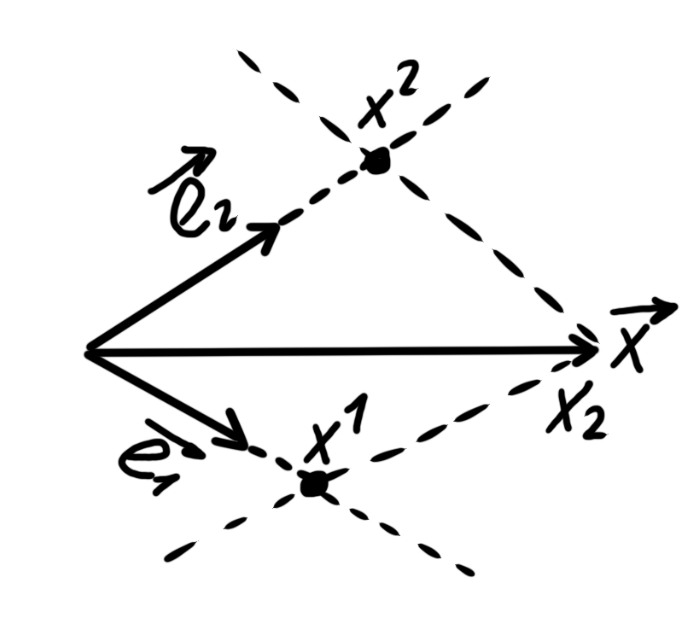
\includegraphics[width=0.4\textwidth]{/Users/vladbelousov/Desktop/Semestr_4-FP-NSU/ЭиО/Лекции_по_дням/image/179.png}
\end{center}

Правило: если два индекса в верхнем и нижнем этажах совпадают, то они называются немыми, это означает по ним ведется суммирование. 

Преобразование Лоренца в тензорном виде: 

\[ \acute{x}^i = L^{i } _{\cdot k}  x^k :\quad  \begin{pmatrix}
    \acute{x} ^0 \\
    \acute{x}^1\\
    \acute{x}^2\\
    \acute{x}^3
\end{pmatrix}  = \begin{pmatrix}
\gamma & - \beta \gamma  & 0 & 0\\
- \beta \gamma & \gamma & 0 & 0\\
0 & 0 & 1 & 0\\
0 & 0 & 0 & 1
\end{pmatrix} \begin{pmatrix}
x^0\\
x^1\\
x^2\\
x^3
\end{pmatrix}\] 
, где \( L_{\cdot k}  ^i  \)  - матрица Лоренца.

Обратное преобразование:

\[ x^i = \overline{L}  ^{i } _{k} :\quad   \acute{x}^k \begin{pmatrix}
    x^0\\
    x^1\\
    x^2\\
    x^3
    \end{pmatrix} = 
        \begin{pmatrix}
        \gamma & \beta \gamma  & 0 & 0\\
        \beta \gamma & \gamma & 0 & 0\\
        0 & 0 & 1 & 0\\
        0 & 0 & 0 & 1
        \end{pmatrix}
        \begin{pmatrix}
            \acute{x} ^0 \\
            \acute{x}^1\\
            \acute{x}^2\\
            \acute{x}^3
        \end{pmatrix}  \] 

Имеем: \( L^{i } _{\cdot k }  (- \beta ) = \overline{L }^i _{\cdot k} (\beta)    \) 

Правило: если четыре величины \( (a^0 , a^1 , a^2 , a^3 ) \) при переходе из \( K \) в \( K'  \) преобразуются через преобразование Лоренца \( \Rightarrow \) это контравариантные компоненты четырех вектора. \\

1. Четырех скаляр (тензор "0" ранга) не изменятся при  преобразование Лоренца; 

2. Четырех вектор (тензор "1" ранга) изменятся \(  \acute{x} ^i = L_k ^i x^k \); 

3. Четырех тензор второго ранга. 

Возьмем два четырех вектора \( (a^0 , a^1 , a^2 , a^3 ) , \text{ }  (b^0, b^1 , b^2 , b^3) \)  и образуем из их компонент 16 велин \( a^i b^k : F^{ik } = \acute{a } ^i  \acute{b } ^k = L^{i }_{\cdot n }   a^n L^k _{\cdot m}  b^m = L^i _{\cdot n}  L^k _{\cdot m}  a^n b^m = F^{nm}  \) \( \Rightarrow  \) правило преобразования тензоров второго порядка: \(  \acute{F} ^{ik }  = L_{ \cdot n} ^i L_{\cdot m}  ^k  \acute{F} ^{nm }  \). 

В матричном виде: \(c_{i j }  = A_{i m }  B_{m j }     \) (произведение двух матриц)
\[  \acute{ F } ^{ik }  = L^i _{\cdot k }  F^{nm }  L^{\top m       } _{\cdot k}  \] 

Тензор третьего ранга: \( \acute{F } ^{ i j k } = L_{ \cdot n }  ^i L_{\cdot m }  ^j L_{\cdot e } ^k F^{nm e}  \)  

\section{Геометрия пространства времени}

\begin{center}
    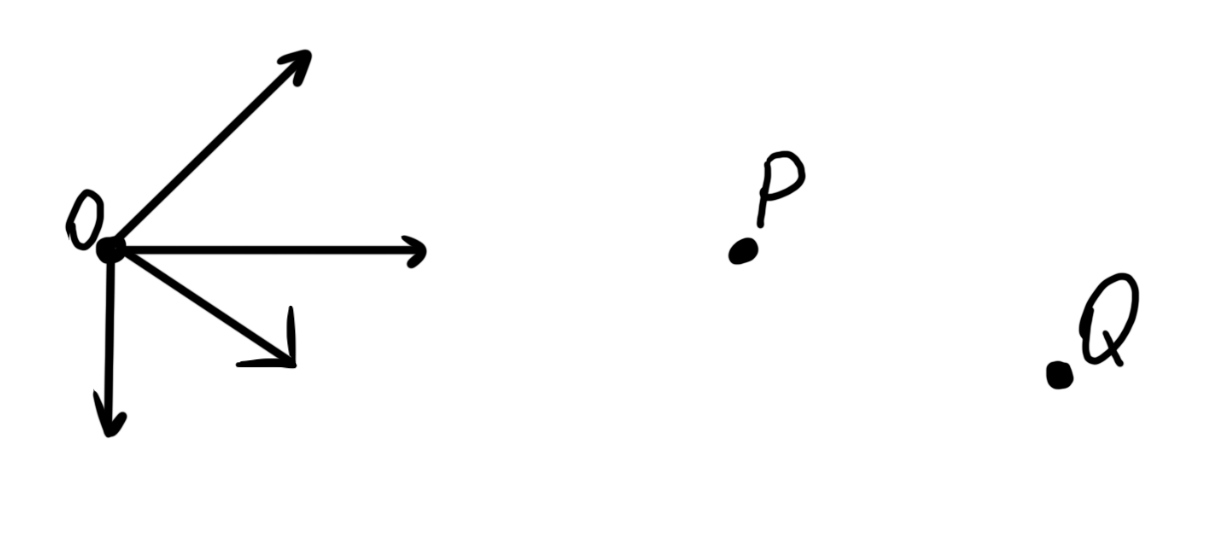
\includegraphics[width=0.6\textwidth]{/Users/vladbelousov/Desktop/Semestr_4-FP-NSU/ЭиО/Лекции_по_дням/image/180.png}
\end{center}

\( e_0 , e_1 ,e_2 ,e_3  \) - четыре любых линейно независимых вектора - образуют базис. 

\[ \vec{ x }  _ p = \overrightarrow{OP } = e_i x^i _ p , \text{ }  \vec{x } _q = \overrightarrow{OQ} = e_i x^i _q   \] 

\( \vec{x} _{pq} =\vec{x } _p - \vec{x }  _q  \)(не зависит от выбора начала отсчета)\( = e_i (x_p ^ i - x_q ^i ) \). Составим скалярное произведение \( (\vec{x } _{pq  }  , \vec{x } _{pq } ) = (e_i (x_p ^i - x_q ^i ) , e_k  ( x_p ^k - x_q ^k )); \text{ }  (e_i , e_k ) \equiv q_{ik } \)  
\[ (\vec{x } _{pq }  , \vec{x }  _{pq }   ) = g_{ik }  (x_p ^ i - x_q ^i ) (x_p ^k - x_q ^k )  = S ^2 = c ^2 (t_p - t_q )  ^2 ( x_p - x_q ) ^2 - (y_p - y_q ) ^2 - (z_p - z_q ) ^2  \] 
Перепишем: \( S ^2 = (x^0 _ p - x^0 _q ) ^2  -(x^1 _ p - x^1 _q ) ^2-(x^2 _ p - x^2 _q ) ^2-(x^3 _ p - x^3 _q ) ^2\) 
\[ \Rightarrow g_{ik }  \text{ - диагональные элементы не равны нулю:  }   \] 
\[g_{i k } =  \begin{pmatrix}
1& 0 & 0 & 0\\
0 & -1 & 0 & 0\\
0 & 0 & -1 & 0\\
0& 0 &0 & -1
\end{pmatrix} \underset{\text{(псевдоэвклидово пространство)} }{\text{ - метрический тензор. } }\] 

В трех мерном пространстве: 

\[ g_{ik }  =\begin{pmatrix}
1 & 0 & 0\\
0 & 1 & 0\\
0 & 0 & 1
\end{pmatrix} \text{ - Эвклидово пространство.} \] 

\[ (e_i ,\vec{x  } ) = (e_i , e_k x ^k )  = g_{i k }  x^k = x_i \text{ - ковариантная компонента } \vec{x}    \] 

\[ (\vec{x }  , \vec{x } ) = (e_i x ^i , e_k x^k ) = (e_i e_k ) x^i x^k = g_{ik }  x^k x^i = x_i x^i  \] 

Правило: \( x_i = g_{ik }  x^k  \)  положено в основу операций с повышением  и понижением индекса.\\

Пример: \( F_{ij k }  = g_{im }  F^m _{\cdot j k}  , \text{ }  F_{i j k }  = g_{im }  g_{j n } g_{ ke }  F^{mnl}  \) 

\[ a^ i = \tilde{ g }^{ik }  a_k , \text{ где  } \tilde{ g }^{ik }  \text{ - обратная матрица к   } g_{ ik}   \] 
\[ g^{ik } \text{ и } g_{ik } \text{ - это метрический тензор }  \begin{pmatrix}
1 & 0 & 0 & 0\\
0 & -1 & 0 & 0\\
0 & 0 & -1 & 0\\
0 & 0 & 0 & -1
\end{pmatrix} \] \\

Пример: \( F^{ij k }  = g^{im } g^{j n }  g^{kl }  F_{mn l}   \)
\[ a^i = g^{ik }  a_k , \text{ }  F^{ij }  = g^{in } g^{jm } F_{nm }  ,\text{ }  F^{i j }  = g^{ in } F_{n \cdot }  ^j     \]  

\textbf{Свойство:} \( g_{ik }  \)  - является инвариантным при преобразование Лоренца.

\[ \acute{g } ^{ik }  = [\acute{ a } ^i \acute{b } ^k = L^i _{\cdot m }  L^k _{\cdot n } a^m b^n ] = L^i _{\cdot m }  L^k _{\cdot n }  g^{mn }  = \text{в матричном виде: } L^{i }  _{\cdot m }  g^{mn }  L^{\top n }_{\cdot k}    \] 

\[ \acute{g } ^{ik }  = \begin{pmatrix}
\gamma   & - \beta \gamma & 0 & 0\\
-\beta \gamma& \gamma  & 0& 0\\
0 & 0 & 1 & 0\\
0 & 0 & 0 & 1
\end{pmatrix} \begin{pmatrix}
1 & 0 & 0 & 0\\
0 & -1 & 0 & 0\\
0 & 0 & -1 & 0\\
0 & 0 & 0 & -1
\end{pmatrix} \begin{pmatrix}
    \gamma   & - \beta \gamma & 0 & 0\\
    -\beta \gamma& \gamma  & 0& 0\\
    0 & 0 & 1 & 0\\
    0 & 0 & 0 & 1
    \end{pmatrix} = \begin{pmatrix}
        1 & 0 & 0 & 0\\
        0 & -1 & 0 & 0\\
        0 & 0 & -1 & 0\\
        0 & 0 & 0 & -1
        \end{pmatrix} \] 

Преобразование Лоренца ковариантных компонент четырех вектора: \\

1-ый способ: \( \acute{x } _i = L _{i \cdot }  ^k x_k \) 
, где \( L^k _{i \cdot}  \) - не матрица Лоренца.

Дописать .

%%-------------------------------%%

% Закрытие документа, если файл компилируется отдельно
\ifdefined\mainfile
    % Если это основной файл, не нужно заканчивать документ
\else
    \end{document}
\fi 